\section{Product Description}
The demand for plant-based food products is growing and the use of plant-based beverages as a substitute for milk has gained popularity. Oat drink has become a popular choice as a milk alternative, leading the food industry to produce an increasing amount \cite*{01_article}. Oat drink is produced as an oat extract from oat flour or rolled oats, resulting in a by-product consisting of insoluble oat components that are not transferred to the oat drink. During production, 86\% of the oats used end up as a by-product \cite*{01_article}. The by-product from the oat production has currently no reuse value in the food industry and is therefore used as animal feed, fertilizer, or biogas \cite*{02_article}.

\vline 

Oats contain several essential amino acids, proteins, and fibers, including beta-glucan, which are valuable nutritional resources, but many of these nutrients are not transferred to the oat drink and thus remain in the oat by-product \cite*{03_article}. By utilizing the by-product of the oat drink production, we can battle food waste by introducing a new and innovative breakfast cereal, with high nutritional value.  

\subsection{Indented Claims and Substantiation}
The innovative breakfast cereal will be produced from upcycled oat pulp, that otherwise would go to waste, the product can therefore be claimed to be sustainable. This is substantiated by sourcing the otherwise wasted oat pulp from the oat drink production sites. The breakfast cereal also have a high nutritional value with a high amount of protein and fiber, including beta-glucan \cite*{03_article}.

\subsection{Consumer and Competitive Analysis}
The breakfast cereal will appeal to multiple different consumer segments. The first target consumer could be the environmentally conscious person who are informed about the impacts of food waste. For these consumers, the sustainability aspect of the breakfast cereal is a major draw. Another target consumer could be the healthy minded people that seek products that are nutritious, high in protein and fiber. For these consumers, the nutritional value of the breakfast cereal is a major draw.  

\vline

Breakfast cereal made from oat are well known products on the marked. For the sustainable segment our product will be unique. There are plenty of organic and “green” products on the marked, but the effort to reduce food waste in the production chain is not clearly marked by other breakfast cereal products. For our nutritional segment, we will have competitors such as Kellogg's All Bran. Kellogg's All Bran and a lot of other brands are focusing on the high fiber content in their cereals. We could brand our self with both high fiber and protein content, plus our additional sustainability qualities, we are sure to stand out.  

\section{Raw Materials}
The main component in this production of cereals is oat pulp. Oat pulp is the by-product after making oat milk \cite*{05_article}. The process is illustrated in figure \ref*{fig:oat_pulp_prod}.

\vline

The first step in the process is to soak the dried oats in water for up to 8 hours. After the soaking process the oats are getting wet milled at a ratio of 1:2,7 (weight/weight). To form a slurry the wet milled oats are treated with enzymes to break down the fibers. To separate the slurry into a fluid fraction and pulp fraction, the slurry is filtrated. It's in this step that the by-product, oat pulp, is made \cite*{05_article}.

\vline

Even though the oat pulp is filtered, it still retains a significant amount of water. This issue is a challenge in terms of microbiological growth and a drying process would extend the shelf life significantly. Furthermore, the drying process will reduce mass which will make it more affordable to transport and decrease the greenhouse gas emission \cite*{05_article}.

\vline

To inhibit spoilage enzymes and microbial growth the water activity should not be higher than 0.6 and the moisture content should not be higher than 10\% \cite*{05_article}.

\vline

The drying temperature is a crucial factor, as it affects the nutritional content, flavour, texture, and color of the product. However, it is also a highly energy-intensive process, potentially accounting for up to 25\% of total production costs. It has been investigated in previous studies that the ideal temperature for oats is between 80-120\textdegree C. The high temperature may lead to a nutrional loss, but also a change in the texture and flavour. The oat pulp could be dried at 80\textdegree C until the right moisture is achieved, $\leq$ 10\% \cite*{05_article}.

\vline

It is desired in this project that the particle size should be around 0.4-0.5 mm to have the optimal size for further production of cereals \cite*{04_article}. The machinery used for milling could be a roller mill, which compresses the oat pulp between a pair of counter-rotating heavy rollers \cite*{04_article}.

\section{Production Process}

Oat pulp is obtained as a by-product of oat milk production. Figure \ref*{fig:oat_pulp_prod} illustrates the side stream in which oat pulp is extracted. While the figure provides an overview of the full oat milk and oat pulp production process, this report will focus on the side stream processing steps (steps 1-7) \cite*{05_article}. 

\begin{figure}[h]
    \centering
    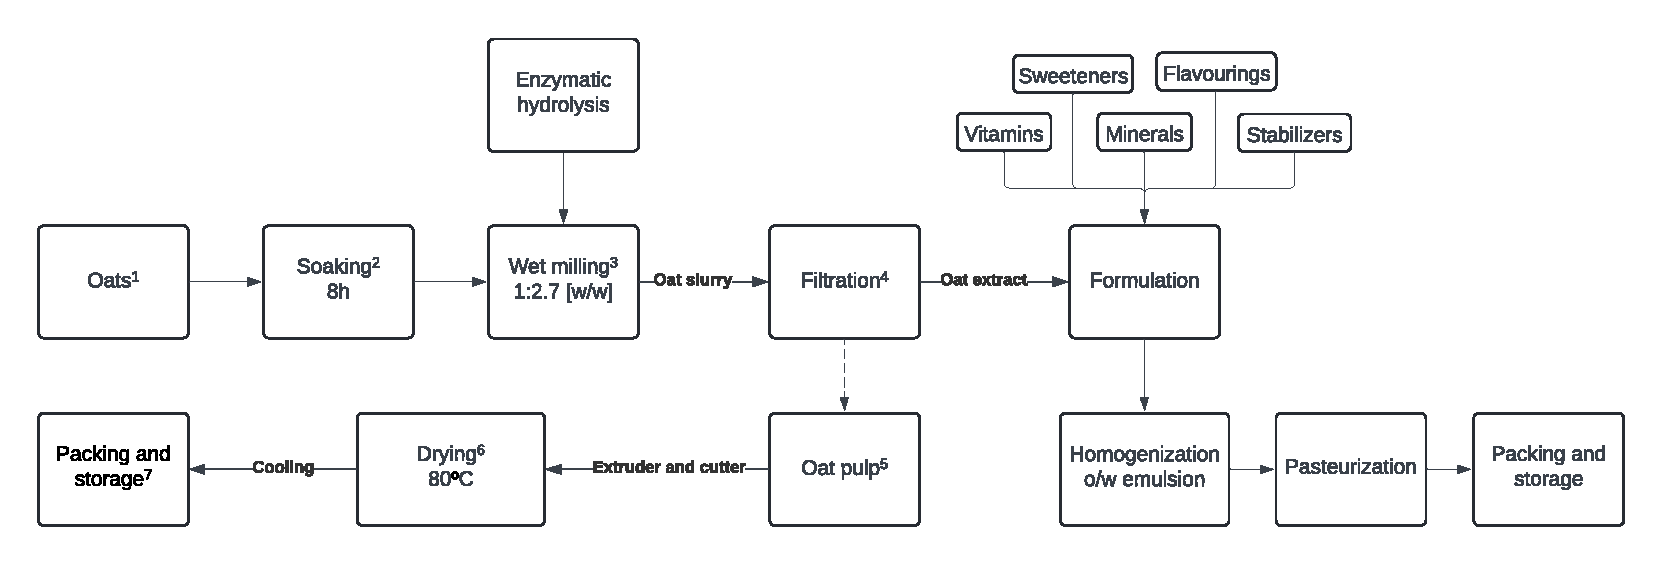
\includegraphics[width=\textwidth]{Figures/oat_pulp_production.pdf}
    \caption{Oat milk and the oat pulp production process as a side stream. The oat pulp is extracted in steps 1-7.}
    \label{fig:oat_pulp_prod}
\end{figure}

\vline

The first step in oat milk production is the hydration of oats. To ensure proper hydration and facilitate further processing, the oats are submerged in water for 8 hours. This soaking process softens the oats and allows for more effective dispersion of enzymes as well as a higher enzymatic activity and better milling, which are crucial for obtaining a homogenous slurry. Without sufficient hydration, the milling process would be less efficient, leading to an inconsistent product with unwanted coarse particles \cite*{05_article}. 

\vline

Following hydration, the next step involves enzymatic hydrolysis and wet milling. Enzymes are added to the soaked oats just before the milling begins. These enzymes primarily break down starches and proteins. The enzymatic treatment helps enhance the flavour and stability of both the oat milk and -pulp extract by reducing raw cereal notes and improving solubility. After hydrolysis, the oats undergo wet milling, where they are ground in a water-to-oat ratio of 1:2.7 (w/w), resulting in a homogeneous oat slurry \cite*{05_article}. 

\vline

Once the milling is complete, the slurry is subjected to filtration to separate the liquid oat extract (used for oat milk production) from the solid oat pulp. The oat extract proceeds through additional processing stages, while the oat pulp is collected for further transformation into cereal \cite*{05_article}. 

\vline

The obtained oat pulp is then pressed through a cold single screw extruder, where it is shaped and cut into small donut-like pieces. Extrusion serves multiple purposes: it provides structural integrity, defines the texture, and ensures even drying in the subsequent step. At this stage, the oat pulp still has a high moisture content, making it unsuitable for long-term storage \cite*{05_article}. 

\vline

To address this, the extruded oat pulp enters the drying process (step 6), where it is dried in an oven at 80°C until the moisture content is reduced to $\leq$10\%. Drying is a critical step as it improves shelf stability, prevents microbial growth, and enhances the crispiness of the final product \cite*{05_article}. 

\vline

Once the drying process is complete, the oat pulp cereal is cooled, packaged, and stored in a controlled environment until it reaches retail stores and end-consumers.

\section{HACCP Analysis}
A HACCP analysis is conducted to ensure food safety by identifying and controlling potential hazards in production. Since our product is a by-product and is not heat-treated but dried, it is crucial to maintain good manufacturing practices. This is achieved through personal hygiene and clear cleaning procedures throughout the production line to prevent contamination. 

\vline

Our raw materials undergo a process where water is added, resulting in a moist mass with high water activity. We aim to reduce water activity as quickly as possible to create an environment that is less favorable for pathogenic bacteria. Drying lowers water activity and thus inhibits microbial growth. To ensure our product remains safe while preserving its structure and minimizing nutrient loss, it is dried at 80\textdegree C. At this temperature and with the required drying time to achieve a moisture content below 10\% and water activity below 0.6, we ensure that pathogenic bacteria such as E. coli, Salmonella, and Bacillus cereus do not survive the process, if present. Therefore, the drying temperature and time is considered a Critical Control Point (CCP), as a lower temperature or too short time could compromise product safety.  To verify safety, samples of both the raw material/by-product and the final product are taken for laboratory testing. If our product does not meet safety standards for consumption, it will be repurposed as animal feed or discarded. 

\vline

In addition to biological hazards, we also focus on physical hazards, such as foreign objects that may not have been removed during the oat milk production process. This is managed by sieving the milled oat to separate any potential contaminants. Before packaging, the product undergoes a metal detector and X-ray screening to ensure it does not contain any unwanted or harmful objects.

\section{Quality Parameters}
The production of oat pulp cereals involves series of steps, and it-is important that these steps are controlled and performed within the desired quality limits. This will ensure that the product contains the aimed characteristics and is safe to consume. The critical quality attributes (CQA) are an overview that gives a valuable input on which quality parameters needed to be adjusted to achieve the desired quality in the product. The following parameters have been identified as the CQA which are: moisture content, nutritional composition and extrusion. 

\subsection*{Moisture Content}
Oat pulp contains a high range of moisture content (54,3 - 65 \%), which is an ideal environment for microbial growth (Le et al., 2025). This means that a pre-drying step is likely required to reduce the moisture content in the range of 20 - 25 \%, which is ideal for the extrusion process. If the moisture content is too high (> 30 \%), it will decrease the expansion process, and the overall structure will fall apart \cite*{RM_magdalena}.

\subsection*{Nutritional Composition}
The breakfast cereal product will mainly consist of significant nutrients from oat pulp. The macronutrients levels of the oat pulp are carbohydrates (12,30 - 27,49 \%), protein (25,71 - 52,10 \%), insoluble fiber (22,97 \%) and soluble fiber (3,19 \%). It is important to ensure that the nutritional profile of the product is not affected by the process in such way that leads to degradation of nutrients \cite*{05_article}.

\subsection*{Extrusion}
The optimal extrusion parameters for oat based cereal breakfast were investigated in Kristiawan et al. (2025). For the extrusion process, the ideal moisture content for oat-based cereals is 20 - 25 \%, which result in effective expansion. Moderate extrusion condition, which includes temperature of 120 C and 100 revolutions per minute increased the soluble fiber by breaking down the insoluble fiber into smaller water-soluble components \cite*{RM_magdalena}.

\section{Sustainability}
The market for plant-based milks has seen rapid growth in recent years, as environmentally conscious consumers shift towards alternatives to traditional dairy products. Especially oat milk is increasing in popularity, exhibiting a growth rate of 350\% in the U.S. with a current total market value of \$424 million. Although oat is a climate friendly substitute for dairy, the production generates a significant side stream of oat pulp, that needs to be utilized to minimize the environmental impact. Each kg of oat milk generates 0.2-0.45kg of oat pulp, meaning that approximately 228 kilotons are produced annually, which is expected to increase to 500 kilotons by 2030. Oat pulp contains a significant amount of plant protein at 25-52\%, making it a contender to replace animal-based protein, which is a primary concern regarding dietary sustainability \cite*{05_article}.

\vline

Plant-based foods are generally associated with high amounts of waste streams, meaning that a shift towards plant-based diets may lead to an increase in food waste, further increasing the need for efficient utilization of side-streams. However, only 5\% of agricultural research investments are targeted towards reducing food waste whereas more than 90\% are spent on increasing crop productivity. Extrusion is emerging as a capable food production technology for food waste valorization and creating novel foods from various industry by-products. The benefits of extrusion include its functionality and versatility as several processing steps such as mixing, heating, shearing, and shaping are combined into a single continuous process that allows various different raw materials to be incorporated and combined. Extrusion has already been applied for a range of by-product-based food products incorporating side streams such as fruit and vegetable pomace, brewer's spent grain, and oil press cakes. Additionally, it is an important technology for manufacturing novel sustainable protein sources like plant-based meat analogues and insect-based foods as it allows for significant manipulation of the textural properties of the product \cite*{06_article}.

\vline

Generally, extrusion is a promising tool for reducing food waste associated with the production of plant-based foods. Utilizing every part of an already climate friendly crop such as oat can facilitate the transition towards a more sustainable food system, ensuring proper nutrition while limiting food waste and environmental impact of the human diet. 
